\chapter{Apresentação de Resultados}
\label{cap:avaliacao_sistema}

Nesse capítulo será feita a apresentação dos resultados obtidos a partir da aplicação do modelo proposto a um cenário.

\section{Introdução}

As discussões nesse capítulo estão descompostas em três partes, sendo elas:

\begin{itemize} \parskip -4pt
    \item \textbf{Fluxo de execução do sistema:} Apresenta a dinâmica do sistema a começar pela leitura dos produtos contidos na geladeira e finalizando na apresentação de recomendações e receitas, além de algumas funcionalidades dentre as descritas no Capítulo 4.
    \item \textbf{Cenário de Aplicação:} Apresenta o cenário através do qual o sistema será avaliado. Assim, detalha-se o ambiente da simulação, os dados utilizados, sua obtenção, organização além das ações executadas pelo sistema.
    \item \textbf{Avaliação do Protótipo:} Nesta seção, a partir do cenário proposto, serão demonstradas interações com o protótipo e o efeito gerado no sistema, seja na forma de recomendações de produtos e receitas, bem como em informações de estado da geladeira e de produtos contidos atualmente.
\end{itemize}

\section{Fluxo de execução do sistema}

No sistema diversas operações são executadas, às quais incluem os diversos componentes do sistema. A seguir, alguns fluxos de execução, dentre os mais relevantes, são apresentados e explanados.

% Demonstrar fluxo de execução da leitura de conteúdo
\subsection{Leitura de conteúdo}

No momento em que a geladeira for ligada, conforme a Figura \ref{fig:cap5_diagr_leitura}, o sistema será inicializado e as portas (ou terminais) serão configurados a fim de permitir a comunicação com os leitores além do mecanismo de fechamento. Ademais, os eventos, engatilhados pela mudança do estado da porta, também são configurados. Após a conclusão das ações mencionadas, o sistema entra em modo de espera.

A partir desse ponto, o sistema dependerá da ação do usuário para operar. Assim, quando o usuário abrir ou fechar a porta, o sensor fechamento irá propagar um novo sinal para o sistema. Quando tal evento de mudança ocorre, verifica-se qual o tipo de evento ocorreu, ou seja, entrada ou saída. Caso aberto, o sistema entra em modo de espera por alguns segundos, garantindo que a porta esteja realmente aberta e reduzindo as chances de ruídos interferirem no funcionamento do leitor. Além disso, garante-se que o usuário tenha tempo suficiente para fechar a porta de maneira voluntária. 

Após o período transcorrer, uma nova leitura é realizada e caso ainda aberta, um registro de porta aberta é enviado ao servidor. 

Caso for verificado, após a interação do usuário, que a porta está fechada, espera-se também alguns segundos. Após esse tempo, um comando de leitura é enviado para os leitores de etiquetas. Estes, por sua vez, realizam a captura das informações das \textit{tags} ao alcance e as enviam ao Raspberry. Por fim, um registro de interação é engatilhado no servidor e gravado na base de interações.

\begin{figure}[htb]
    \caption{Leitura de conteúdo da geladeira}
    \label{fig:cap5_diagr_leitura}
    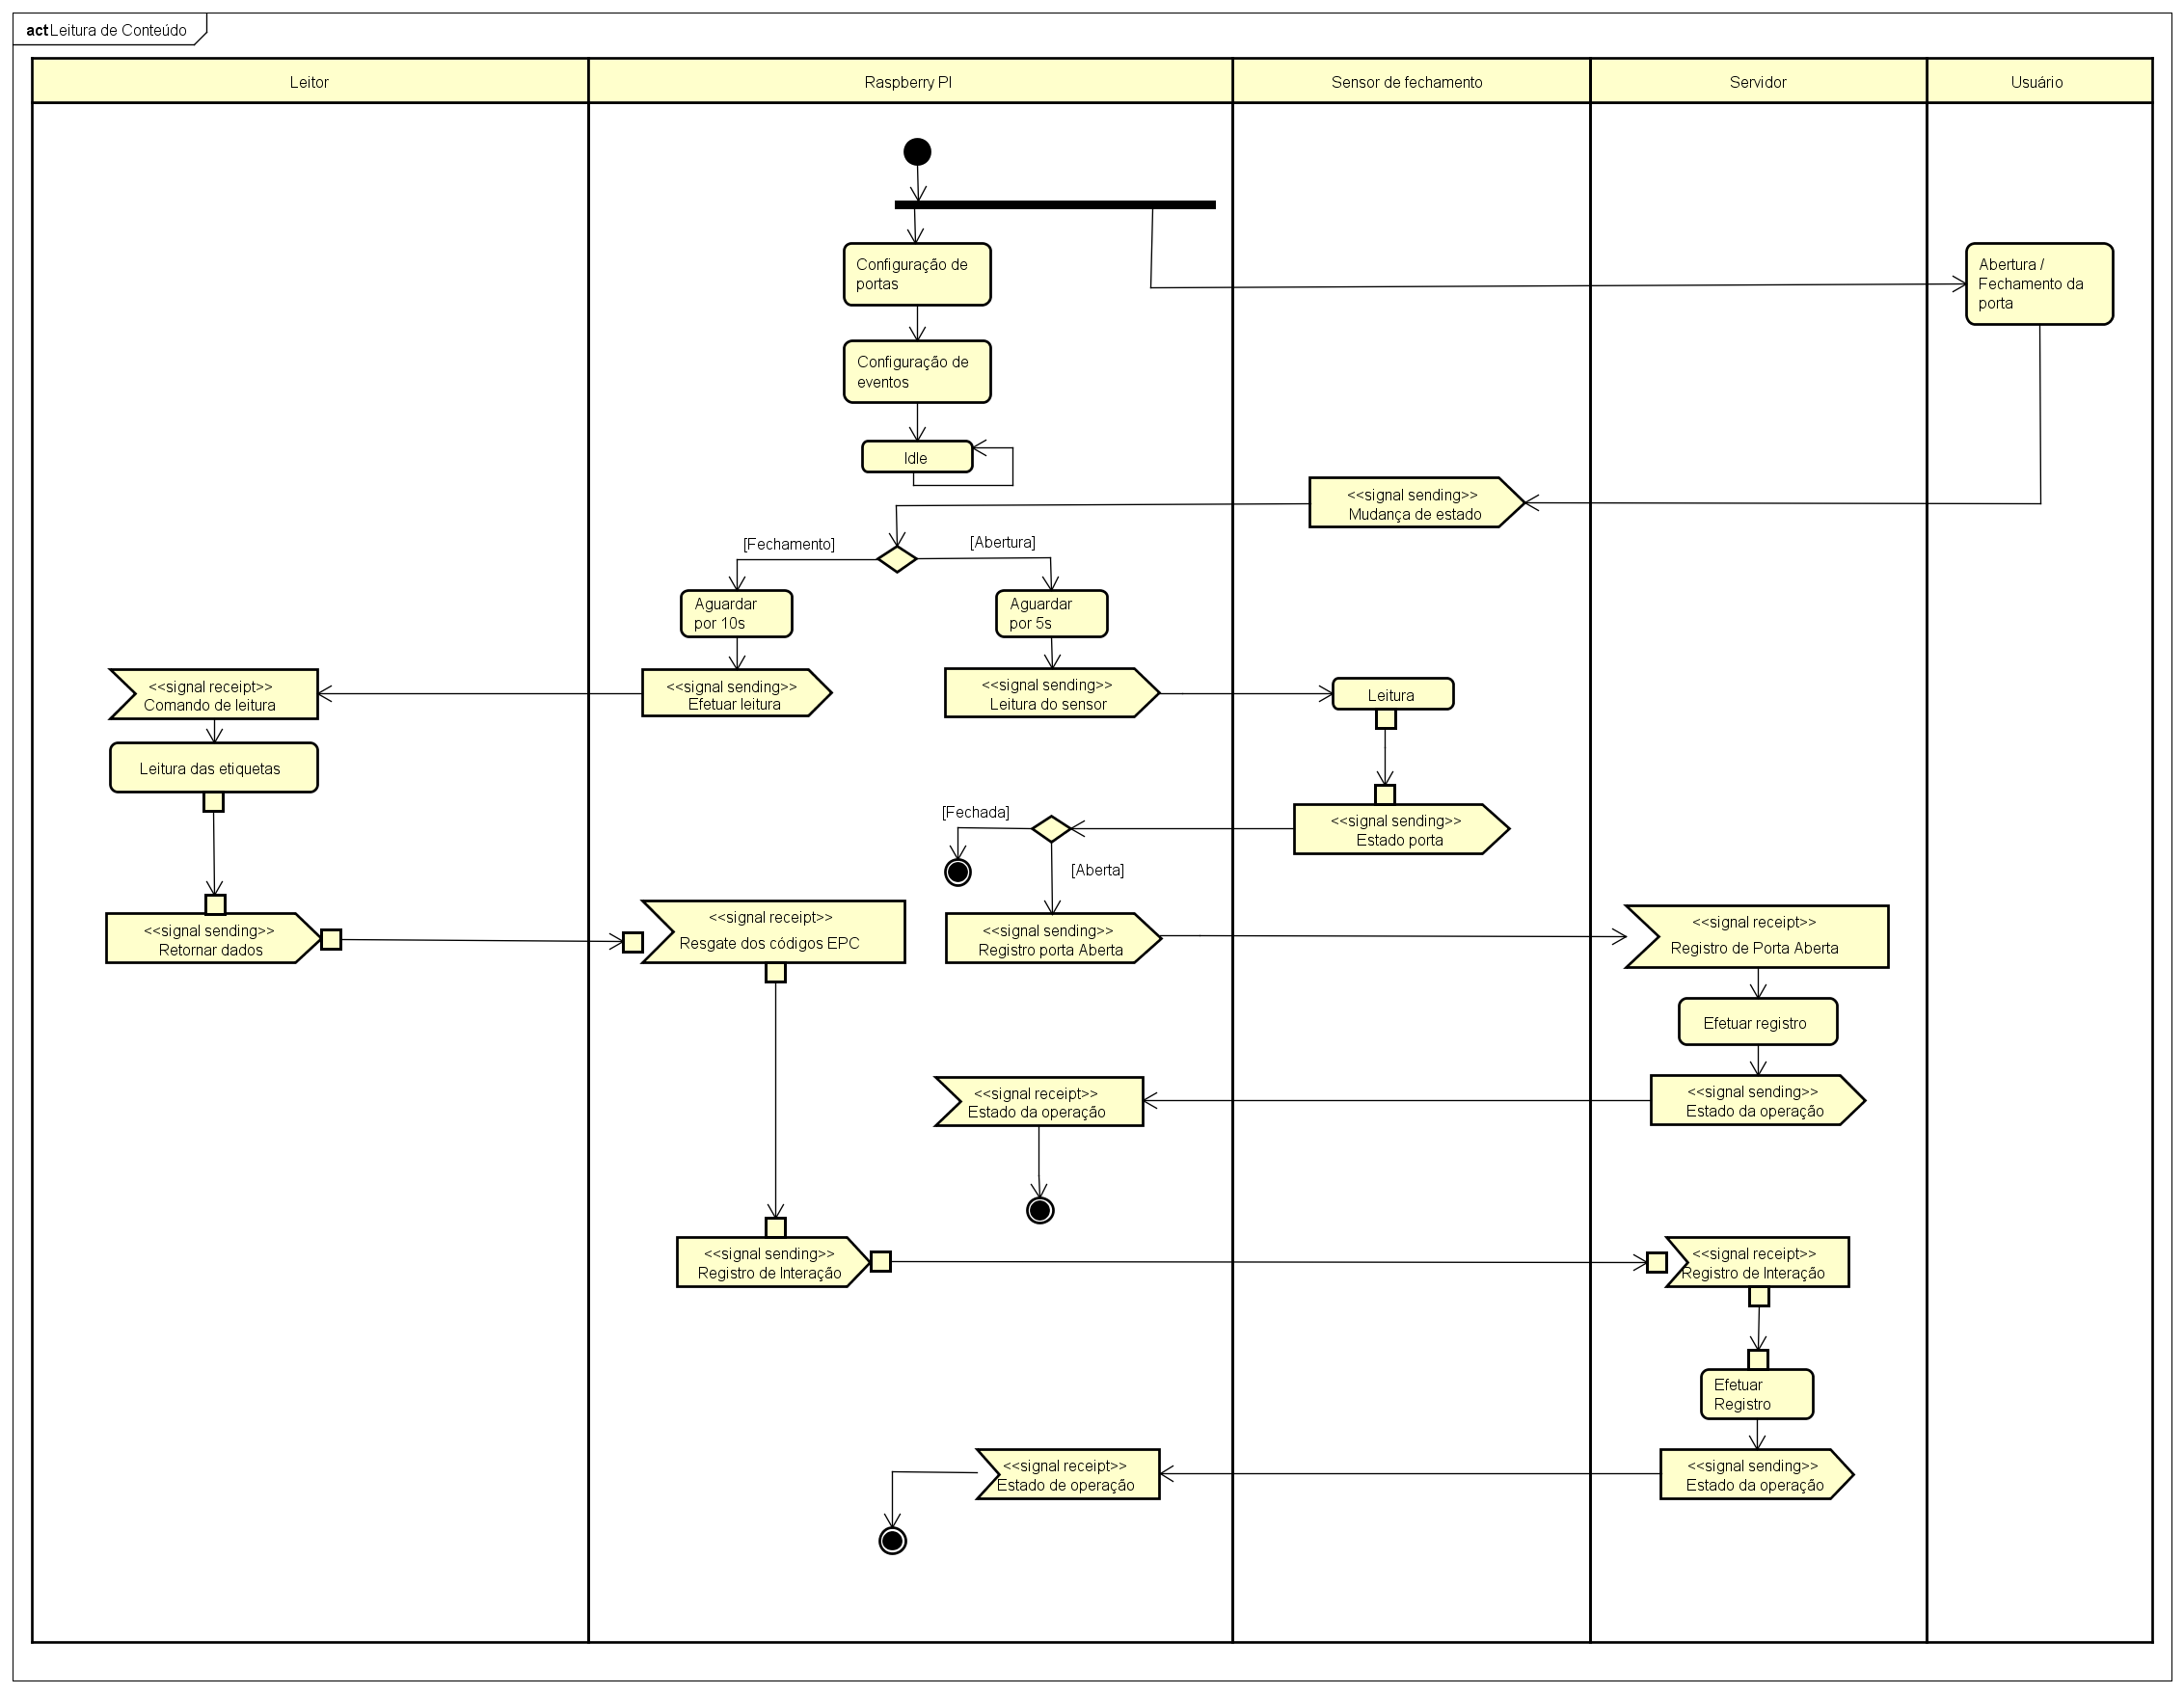
\includegraphics[width=\textwidth]{diagramas/diagr_leitura.png}
    
    \footnotesize{Fonte: Autor}
\end{figure}

\subsection{Listagem de conteúdo da geladeira}

Como uma continuação do processo anterior, o processo de listagem de produtos disponibiliza na interface o conjunto de produtos disponíveis. A Figura \ref{fig:cap5_diagr_lista_prod} demonstra o fluxo de atividades para este processo.

O gatilho para tal ação é dado na interface e esta enviará uma requisição da lista de produtos referentes à uma geladeira específica. Ao receber a solicitação, o servidor fará uma busca na base de interações pelo último registro gravado ao qual contém os códigos EPC lidos das etiquetas. Após isso, tendo o conjunto de códigos EPC, fará uma busca pelo produto correspondente a cada um. Assim, se terá uma lista de produtos e suas respectivas quantidades. Por fim, a lista de produtos, em formato JSON, é retornada à interface e apresentada ao usuário.

% Demonstrar fluxo de execução de listagem de produtos
\begin{figure}[htb]
    \caption{Listagem de conteúdo da geladeira}
    \label{fig:cap5_diagr_lista_prod}
    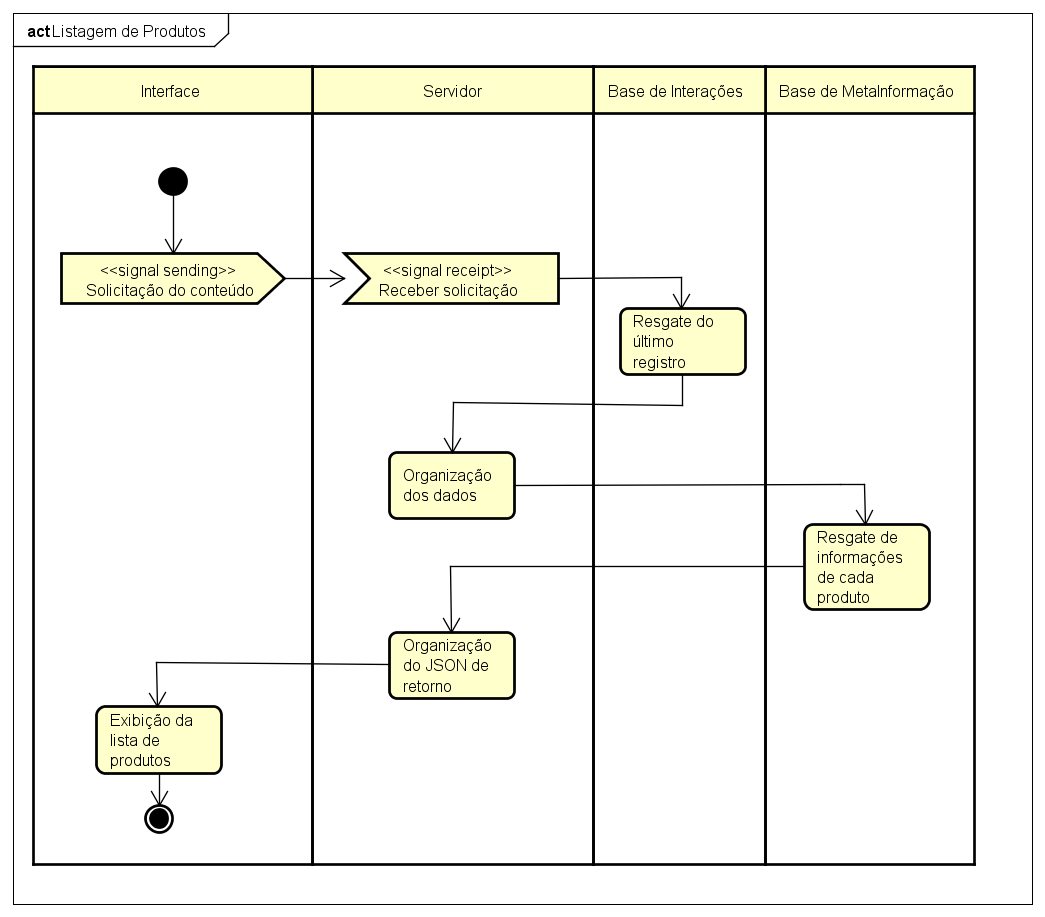
\includegraphics[width=\textwidth]{diagramas/diagr_lista_prod.png}
    
    \footnotesize{Fonte: Autor}
\end{figure}

\subsection{Geração de Recomendação de Produtos Novos}

O processo de geração de recomendações, como já dito, é automaticamente inicializado pelo servidor, conforme Figura \ref{fig:cap5_diagr_geracao_rec}. Inicialmente, a matriz de frequência de interações de usuários com produtos é criada. Vale destacar, que um usuário se refere à uma geladeira. Em seguida, busca-se, na base de interações, todas as interações armazenadas. A partir das interações, na base de metainformação é feita a combinação entre códigos EPC e código de barras. A matriz de frequências é, então, preenchidas com os dados obtidos no processo anterior.

Como parte do cálculo da correlação de Pearson, a média de interações de cada usuário deve ser calculada. Logo após, é computada a similaridade entre os pares de usuários, indicados na Figura \ref{fig:cap5_diagr_geracao_rec} como $U1$ e $U2$, com a Equação \ref{eq:correlacao-pearson}.

Em posse das similaridades entre usuários, inicia-se o processo de recomendação para cada usuário ($U1$) cadastrado no sistema. Inicialmente, o conjunto de similaridades do usuário $U1$ com os demais é ordenado em ordem decrescente, ou seja, do usuário com maior similaridade ao menor. Em seguida, para cada usuário $U2$ na lista de similaridades é feita uma subtração de conjuntos de produtos aos quais $U2$ interagiu pelos que $U1$ o fez. Assim, tem-se um conjunto de produtos que $U1$ não conhece e que poderão ser sugeridos como novas opções de compra. 

O processo citado é repetido até que todos os usuários na lista de similares forneçam recomendações ou quando o número máximo de produtos recomendados for atingido. E, quando uma das duas possibilidades ocorrer, o conjunto de recomendações será salvo na base de recomendações e o o processo de recomendação se repetirá para o próximo usuário.

% Demonstrar fluxo de execução de geração de recomendação
\begin{figure}[H]
    \caption{Geração de Recomendações}
    \label{fig:cap5_diagr_geracao_rec}
    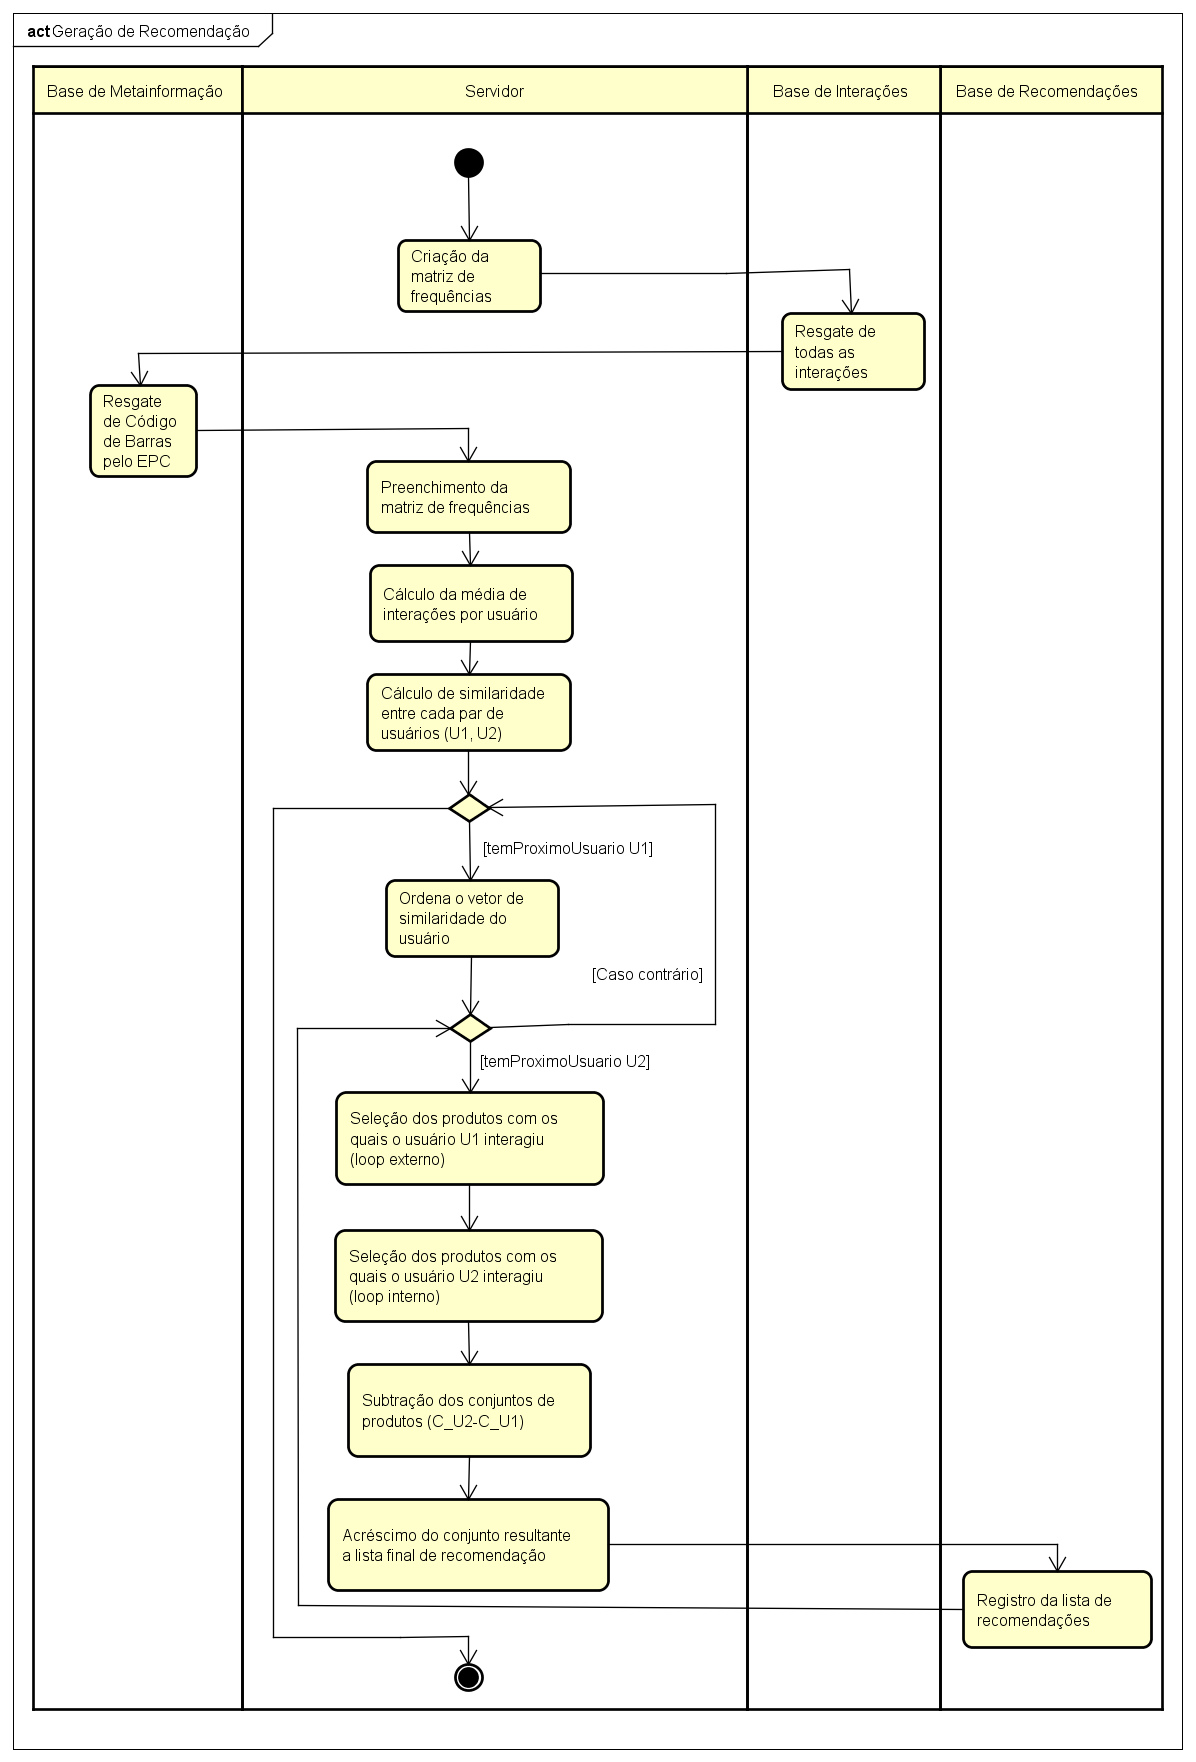
\includegraphics[width=\textwidth]{diagramas/diagr_geracao_rec.png}
    
    \footnotesize{Fonte: Autor}
\end{figure}

\subsection{Listagem de Recomendações}

O processo de listagem de recomendações é engatilhado na interface de usuário. Desse modo, a interface envia uma requisição ao servidor solicitação um conjunto de recomendações para um determinado usuário, conforme Figura \ref{fig:cap5_diagr_lista_rec}.  Ao receber a solicitação, o servidor, faz uma busca na base de recomendações pelos produtos recomendados. Em seguida, os dados são organizados e o conjunto de recomendação é enviado à interface.

% Demonstrar fluxo de execução de listagem de recomendação
\begin{figure}[htb]
    \caption{Listagem de Recomendações}
    \label{fig:cap5_diagr_lista_rec}
    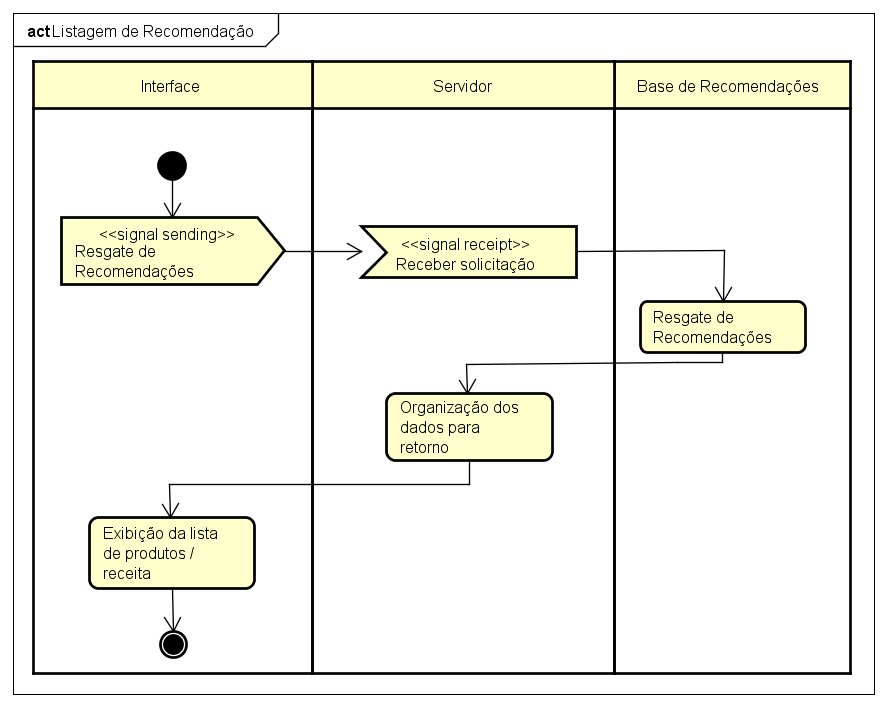
\includegraphics[width=\textwidth]{diagramas/diagr_list_rec.png}
    
    \footnotesize{Fonte: Autor}
\end{figure}

% Demonstrar fluxo de execução de listagem de produtos

\section{Cenário de Aplicação}

A avaliação do modelo dar-se-á a partir do ambiente ilustrado na Figura \ref{fig:cap5_ambiente-cenario}. O ambiente consiste na demonstração de uma sequência de ações, começando pela interação do usuário, com o objetivo de observar o efeito no protótipo implementado.

\begin{figure}[htb]
    \caption{Ambiente do cenário}
    \label{fig:cap5_ambiente-cenario}
    \includegraphics[width=\textwidth]{figuras/cap5_cenario.png}
    
    \footnotesize{Fonte: Autor}
\end{figure}

Em relação, as bases de dados, essas foram preenchidas antes da avaliação do sistema. 
% Descrição dos dados de produtos
Primeiramente, para a base de metainformação foram alocadas informações de quarenta (40) produtos, extraídas dos produtos originais em um supermercado em Araranguá. Excetua-se apenas o endereço URL da imagem de cada produto ao qual foi obtido web-sites de supermercados. 
% Descrição de dados de receitas
Já em relação às receitas, utilizou-se de dez (10) receitas obtidas a partir de sites de culinária. Tanto informações  de produtos quanto receitas foram formatadas conforme a Seção \ref{sssec:metainfo}.

% Descrição da quantidade de usuários
Quanto à identificação das geladeira e, por consequência, dos usuários, não criou-se uma base específica para eles, apenas atribuiu-se um identificador utilizado em cada registro específico a um determinado usuário. Como definiu-se dez (10) geladeiras, foram definidos os valores de um (1) a dez (10) para diferenciação de cada uma.

% Descrição da quantidade de interações por usuários.
Para cada geladeira, foram criadas, de maneira aleatória, interações, cada qual com um conjunto de códigos EPCs representandos os produtos. Assim, definiu-se que o número de interações seria maior ou igual a cinco (5) e menor ou igual a 25. Além disso, para cada interação o número mínimo de itens registrados seria de três (3) e, no máximo, 10.

% Configurações de produtos
Em relação às configurações, descritas na Seção \ref{sssec:base_est-aux}, todos as geladeiras apresentaram parâmetros idênticos excetuando-se as listas de produtos essenciais e suas respectivas quantidades mínimas. Assim, quais produtos e quais quantidades foram definidas randomicamente. Quanto à quantidade de produtos requisitados, estabeleceu-se o número de cinco (5) produtos e, em relação à quantidade, definiu-se um valor randômico entre um (1) e vinte (20).

% Quais os produtos que têm RFID que serão usados na geladeira
Como forma de teste do protótipo da estrutura física da geladeira, três produtos receberam etiquetas com o respectivo código EPC. Sendo eles...
% TODO:  Especificar os produtos


%%%%%%%%%%%%%%%%%%%%%%%%%%%%%%%%%%%%%%%%%%%%%%%%%%%%%%%%%%%%%%%%%%%%%%%%%%%%%%%%%%%%%%%%%%%%%%%%%%%%%%%%%%%%%%%%%%%%%%%%%%%%%%%
\section{Avaliação do Protótipo}

\subsection{Leitura e exibição do conteúdo}
 Inicialmente a geladeira está vazia.
 Ao colocar dois produtos, sendo eles, o ``Margarina com Sal Qualy'' e ``Creme de Leite Tirol'', respectivamente, depois de alguns minutos os seguintes códigos EPC são lidos.
 
 \begin{itemize} \parskip -3pt
     \item 8665580279609348107299713701
     \item 8665580277303506451141610373
 \end{itemize}
 
 Os dados são, então, enviados ao serviço de registro de interação e o seguinte registro é gravado na base de interações. 
 
 \begin{figure}[htb]
     \caption{Registro de interação dos produtos}
     \label{fig:cap5_registro_interacao}
     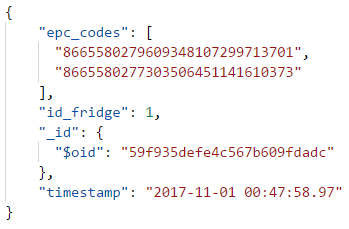
\includegraphics[width=0.5\textwidth]{cap5_registro_interacao}
 \end{figure}
 
 %%%%%%%% JSON DO REGISTRO  %%%%%%%%
 
Ao tentar ler o conteúdo da geladeira logo após o fechamento da porta, a listagem da interface continua sendo vazio. Alguns segundos depois, a listagem é atualizada e o conteúdo exibido é mostrado na Figura \ref{fig:cap5_listagem_atual}.

\begin{figure}
    \caption{Listagem de produtos na Interface}
    \label{fig:cap5_listagem_atual}
    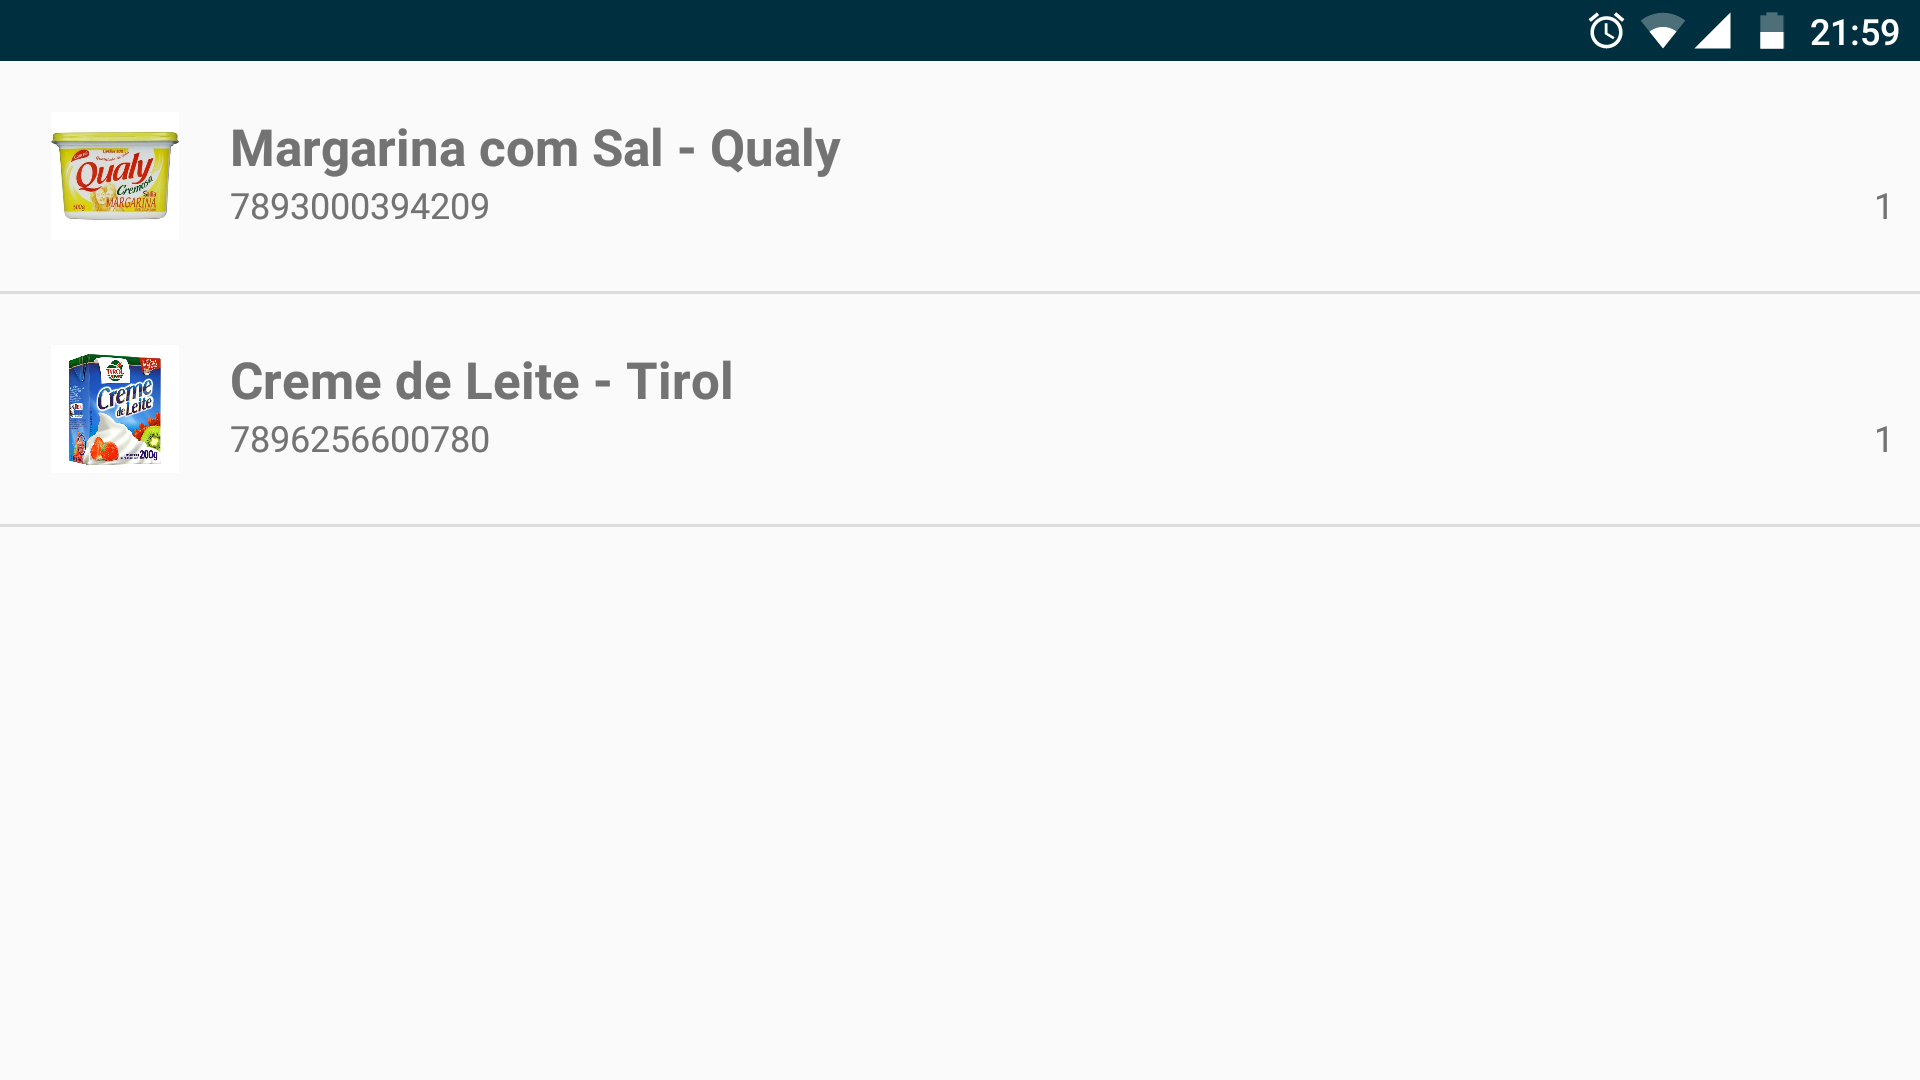
\includegraphics[width=0.8\textwidth]{cap5_listagem_atual}
\end{figure}
 
 %%%%%%%%%%%%%%%%%%%%%   FIGURA DA LISTAGEM APÓS A INTERAÇÃO %%%%%%%%%%%%%%%%%%%%%%%%%%%%%%%%%%%
 
 Dessa forma, afirma-se que a listagem de produtos está operando de acordo com o esperado, já que a lista é alterada após a interação. No entanto, o fator temporal entre a interação e a exibição é compreensível. Assim, o intervalo de tempo decorre do aguardo, na geladeira, até a realização da leitura. Como descrito na Seção X, isso é necessário para garantir que o usuário não coletará novos itens.

\subsection{Geração de Recomendações de Produtos Novos}


Deseja-se gerar recomendações para o Usuário 1. Para tanto, executou-se o cálculo de similaridade entre usuários sobre a matriz de frequências de interações e obteve-se o usuário mais semelhante. Tal indivíduo é identificado como Usuário X e o grau de similaridade entre este o Usuário 1 foi de 0.00.

%inicia-se com a criação da matriz de frequências seguida pelo resgate das interações e, a partir dessas, dos códigos de barras e, por fim o preenchimento da matriz, conforme Figura \ref{fig:cap5_diagr_geracao_rec}.

Como forma de verificação, tem-se as seguintes linhas da matriz de frequência, referentes aos usuários.

%%%%%%%%%%%%%%%%%%  MATRIZ  %%%%%%%%%%%%%%%%%%%%%%

Executando o cálculo da correlação de Pearson, descrita na Equação \ref{eq:correlacao-pearson}, tem-se

%%%%%%%%%%%%%%%%%%  EQUAÇÃO COM VALORES SUBSTITUÍDOS  %%%%%%%%%%%%%%%%%%%%%%%%%%%%%%

Assim, demonstra-se que o cálculo de similaridade está correto.

Percebe-se que o número de produtos com os quais o Usuário 1 não apresentou nenhuma interação, ou seja, as posições na linha do usuário mencionado não estão preenchidas, é XX. Assim, espera-se que pelos menos esses produtos sejam recomendados. 
No entanto, um número maior de itens podem ser sugeridos. Isso ocorrerá quando a quantidade obtida de recomendações através do usuário, com maior similaridade, for insuficiente. Assim, recomendações de outros usuários, com graus de semelhança menores, serão consideradas.

Obteve-se a seguinte lista de itens como recomendação.

 %%%%%%%%%%%%%%%%%%%%%   FIGURA DA LISTAGEM DE RECOMENDAÇÕES DE PRODUTOS NOVOS %%%%%%%%%%%%%%%%%%%%%%%%%%%%%%%%%%%

Como esperado, a lista contém os produtos recomendados pelo usuário com maior similaridade, além de outros, sugeridos a partir de outros usuários.

\subsection{Geração de Recomendações de Produtos Faltantes}

Nessa seção, busca-se avaliar a recomendação da reposição de produtos aos quais o usuário julga serem essenciais a ele. Para tanto, considera-se o conjunto de produtos contidos atualmente:

%%%%%%%%%%%%%%% Lista de um conjunto de produtos atuais %%%%%%%%%%%%%%%

E o conjunto de produtos ditos essenciais:

%%%%%%%%%%%%%%% Lista de um conjunto de produtos essenciais %%%%%%%%%%%%%%%

Percebe-se que alguns produtos estão ausentes e, outros, em falta como, por exemplo, os produtos X e Y, estão em quantidades insuficientes e os produtos A e B estão ausentes. Assim, a recomendação deve conter tais produtos além de outros não citados.

Como sugestões, foram apresentados os seguintes produtos na interface de usuário.

%%%%%%%%%%%%%%% Lista de um conjunto de produtos recomendados %%%%%%%%%%%%%%%

Percebe-se que há uma diferenciação entre os produtos, sendo elas a ``Reposição'', ``Novo'', ``Similar''. A reposição trata da recolocação de produtos essenciais, já o novo, à recomendação de produtos novos, como descrito anteriormente, mas que o usuário decide se deseja seguir a sugestão e comprar tais itens. O ``Similar'' indica a reposição de produtos essenciais que não estavam disponíveis no mercado, mas que foram substituídos por produtos idênticos. Por exemplo, uma caixa de leite da marca X foi substituída por outra caixa de leite, mas da marca Y.

\subsection{Geração de Recomendações de Receitas a partir de Conteúdo}

A recomendação de receitas por conteúdo, como descrito na seção respectiva no Capítulo 4, busca disponibilizar um conjunto de receitas ao usuário, de acordo com os itens que este possui em sua geladeira. 

Considera-se que, inicialmente, os seguintes produtos estejam disponíveis, e suas respectivas quantidades:

\begin{itemize} \parskip -3pt
    \item ABC com X itens
    \item DEF com Y itens 
    \item GHI com Z itens
    \item JKLM com w itens
\end{itemize}

O processo de recomendação avaliará os produtos do ponto de vista de suas características, ou seja, terá um enfoque nos tipos de produtos e não em produtos de determinadas marcas. Assim, avalia-se que se tem X+W caixas de leite, Y doce de leite e Z pacotes de bife e as receitas selecionadas deverão conter no mínimo um desses produtos.

O processo de recomendação avaliação quais receitas satisfazem o requisito especificado e retornará um conjunto de itens para sugestão.

Os itens sugeridos como recomendações são mostrados na Figura X.

%%%%%%%%%%%%%%%%%%    FIGURA X (Lista de receitas de recomendação)    %%%%%%%%%%%%%%%%%%%%%%%%%%%%%

Ao selecionar a primeira receita, tem-se a visão da Figura Y.

%%%%%%%%%%%%%%%%%%    FIGURA Y (Detalhe da receita)    %%%%%%%%%%%%%%%%%%%%%%%%%%%%%

Dos produtos contidos, X itens estão presentes nessa receita, conforme mostrado.
Além disso, ao observar as demais receitas sugeridas, constata-se a conformidade com o conjunto de produtos disponíveis.

\subsection{Geração de Recomendações de Receitas por perfil}

Como descrito na seção X, a sugestão de receitas por perfil buscará receitas que contenham alguns dos itens com os quais o usuário mais interagiu. Para tanto, uma matriz de frequência de interações é montada.  Com base nas frequências de interações do usuário em questão, uma lista é criada a partir dos tipos de produtos existentes.

Considerando-se que os seguintes produtos estejam contidos:

\begin{itemize} \parskip -3pt
    \item ABC
    \item ABC
    \item ABC
    \item ABC
\end{itemize}

E a lista geradas a partir do conjunto anterior seja a seguinte:

\begin{itemize} \parskip -3pt
    \item Caixas de leite
    \item Leite condensado
    \item Carne
    \item Refrigerante
\end{itemize}

Com base em tal conjunto, o processo de recomendação fez uma busca na base de interações pela receitas que contivessem tais categorias de produtos. A partir disso, o conjunto de receitas da Figura X, foi sugerido.

%%%%%%%%%%%%%%%%%%%%%% FIGURA CONJUNTO DE RECEITAS %%%%%%%%%%%%%%%%%%%%

Ao selecionar a primeira receita, tem-se:

%%%%%%%%%%%%%%%%%%%%%% FIGURA RECEITA SUGERIDA %%%%%%%%%%%%%%%%%%%%

\subsection{Alerta de Porta Aberta}

%% OBJETIVO
Os alertas ao usuário que esquecem a porta da geladeira aberta, ou não a fecham corretamente, é importante para evitar gastos desnecessários com energia e, possivelmente, com alimentos estragados. Como descrito na seção X, o processo de verificação de porta aberta, engatilha um registro no servidor. Considerando que, inicialmente, a porta estava fechada e, em dado momento, foi deixada aberta.

Após alguns segundos o seguinte registro foi feito na base de estruturas auxiliares, informando a situação.

%%%%%%%%%%%%%%%%% REGISTRO DE PORTA ABERTA  %%%%%%%%%%%%%%%

Algum tempo depois, a interface fez uma requisição ao serviço de estado de porta. Nesse caso, a aplicação da interface verificou que o estado era aberto e notificou ao usuário, conforme a Figura X.

%%%%%%%%%%%%%%%%% IMG NOTIFICAÇÃO DE PORTA ABERTA  %%%%%%%%%%%%%%%

